\documentclass[10pt,a4paper]{article}
\usepackage[utf8]{inputenc}
\usepackage{amsmath}
\usepackage{graphicx}
\usepackage{amsfonts}
\usepackage{amssymb}
\usepackage{hyperref}
\usepackage{breakurl}
\author{Qin ZHOU \\
    fatestudio@gmail.com
    \and
    Liang XIA \\
    liangxia2006@gmail.com
    }
\title{CS240A Project: Parallelized Attacks on Elliptic Curve Discrete
Logarithm Problem}
\begin{document}
\maketitle

\section{Abstract}
\indent The infeasibility of Elliptic Curve Discrete Logarithm Problem (ECDLP) guarantees the security of all Elliptic Curve based cryptography. There are many attacking methods towards ECDLP to degrade this infeasible problem, among them Pollard $\rho$ method is the best general method known so far\cite{CERTICOM}. In this project, we generate many elliptic curves according to our demand, then develop two algorithms: naive bruteforce algorithm and Pollard $\rho$ algorithm, and parallelized both algorithms. After that we tested all algorithms and evaluated the power of parallelization. 

\section{Introduction}
\indent Elliptic Curve Cryptography (ECC) is a new public-key technology that offers performance advantages at higher security levels. ECC can be applied into many public-key protocols, e.g., an Elliptic Curve version of the Diffie Hellman key exchange protocol (ECDH)\cite{DH1976}, Elliptic Curve Digital Signature Algorithm (ECDSA)\cite{ecdsa-cert} and Elliptic Curve
   versions of the ElGamal Signature Algorithm \cite{E1985}. These protocol prototypes build the foundation of current computer security.\\ 
   \indent ECC uses much less bits while achieving the same level of security compared to RSA (160 bits of ECC provide the same security as 1024 bits of RSA), which means less bandwidth usage and better performance. Figure~\ref{table:nist} gives the bit number of ECC and RSA at the same level of security. \\
\begin{figure}[h!]
  \centering
    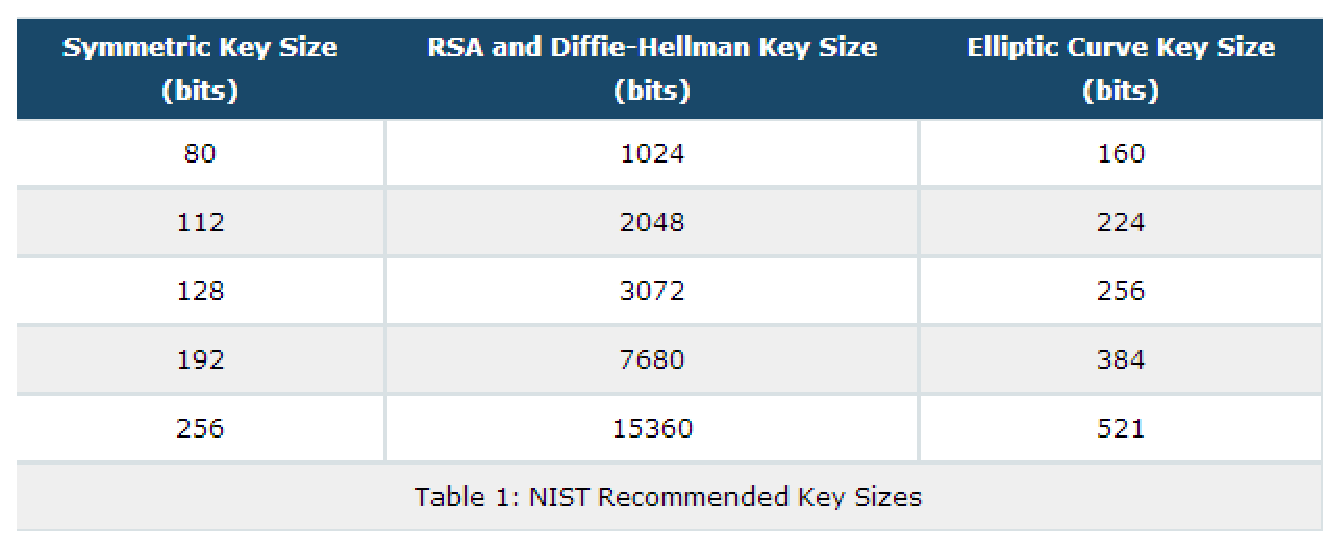
\includegraphics[scale=0.5]{nist.eps}
  \caption{Bit number of ECC and RSA at same level of security}
  \label{table:nist}
\end{figure}
   \indent The adoption of ECC has been slower than had been anticipated, perhaps due to the lack of freely available normative documents and uncertainty over intellectual property rights\cite{RFC6090}. 
   
\section{Elliptic Curve Cryptography}
\indent An elliptic curve $E$ is the graph of an equation
$$ E: y^2 = x^3 + ax^2 + bx + c $$
where $a$, $b$, $c$ are in whatever is the appropriate set (rational numbers, real numbers, integers mod a prime, etc). \\
\indent There are many different families of elliptic curves, among which we define our elliptic curves below:
$$ E = \{(x, y) | x,y \in \mathbb{F}_p, y^2 = x^3 + ax + b\} $$
\indent Where $x$, $y$, $a$, $b$ are in finite field $\mathbb{F}_p$, $p$ is a prime number. We choose $a$ and $b$ randomly and they satisfy the equation below to make the curve non-singular: $$ 4a^3 + 27b^2 \equiv 0\ (mod\ p) $$
\indent After the definition of elliptic curve $E$, we define the addition operation on points of $E$:\\
\indent Suppose two points $P_1 = (x_1, y_1) \in E$ and $P_2 = (x_2, y_2) \in E$, define addition operation:
$$ P_3 = (x_3, y_3) = P_1 + P_2 = (x_1, y_1) + (x_2, y_2) $$
where $$ x_3 = m^2 - x_1 - x_2 $$
$$ y_3 = m(x_1 - x_3) - y_1 $$
and 
$$m = \left\{
	\begin{array}{l l}
    	(y_2 - y_1)/(x_2 - x_1) & \quad P_1 \neq P_2\\
    	(3x_1^2 + b)/(2y_1) & \quad P_1 = P_2
  	\end{array} \right.$$\\
\indent If the slope $m$ is infinite, then $P_3 = \infty$. There is one additional law: $\infty + P = P$ for all points $P$.\\
\indent We add another point $\infty = (\infty, \infty)$ into this curve $E$, then the points of $E$ form an \textbf{abelian group}. Abelian group is the key component of cryptography. \\
\indent Here is the intuition of the addition equation above: Draw the line $L$ through $P_1$ and $P_2$ (if $P_1 = P_2$, take the tangent line to $E$ at $P_1$). The line $L$ intesects $E$ in a third point $Q$. Reflect $Q$ through the $x$-axis (i.e., change $y$ to $-y$) to get $P_3$. Figure~\ref{table:p1p2_1} and Figure~\ref{table:p1p2_2} illustrate the addition operation on an elliptic curve\cite{ECC Book}.
\begin{figure}
\begin{minipage}[width=0.5\linewidth]{0.5\linewidth}
  \centering
    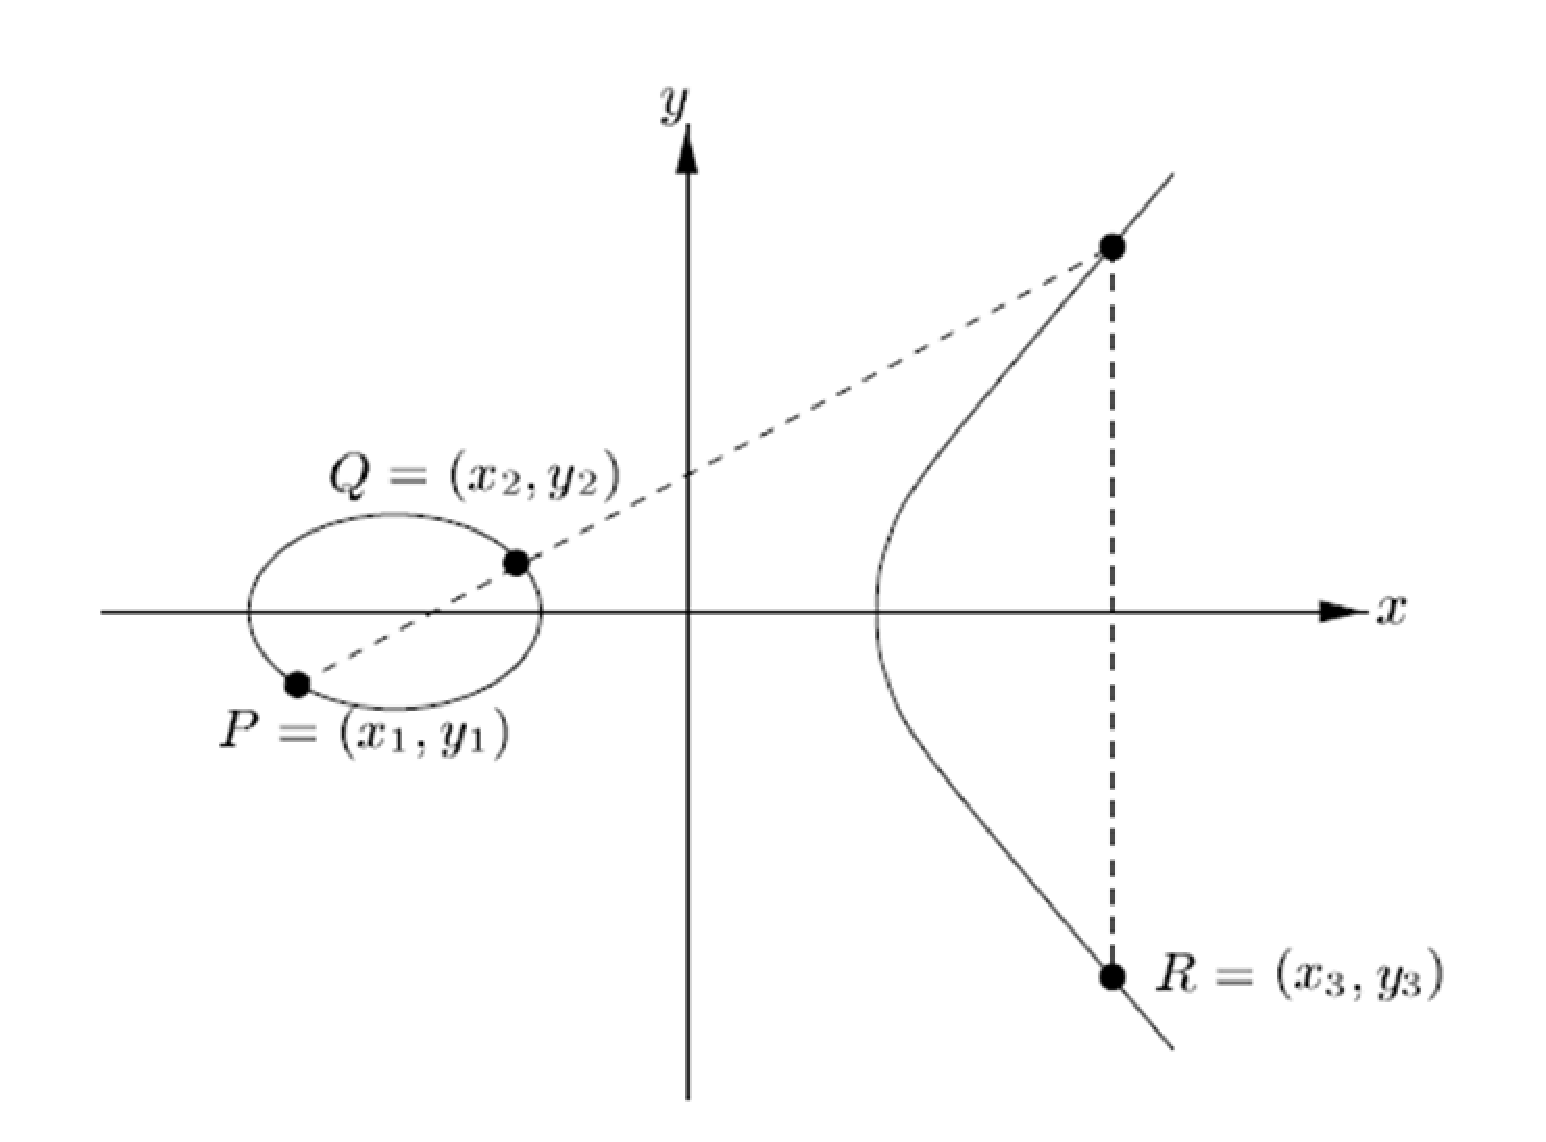
\includegraphics[scale=0.3]{p1p2.eps}
  \caption{$P + Q = R\ (P \neq Q)$}
  \label{table:p1p2_1}
\end{minipage}
\begin{minipage}[width=0.5\linewidth]{0.5\linewidth}
  \centering
    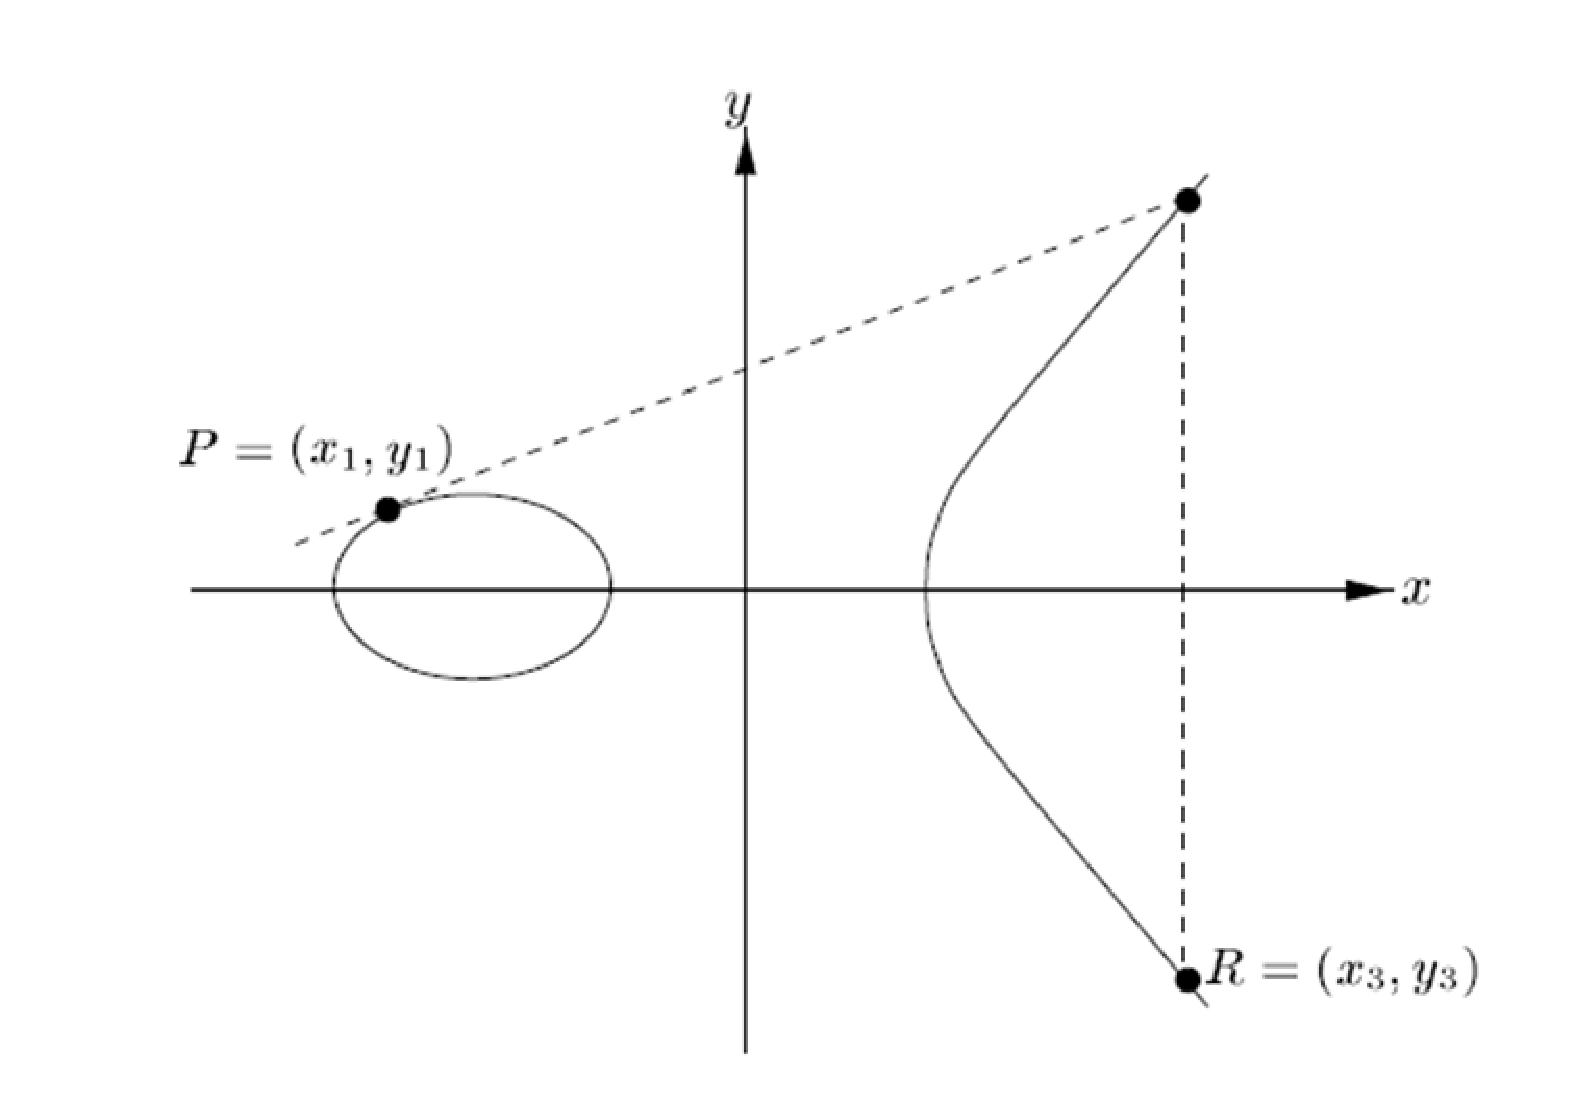
\includegraphics[scale=0.3]{2p.eps}
  \caption{$P + P = 2P = R$}
  \label{table:p1p2_2}
\end{minipage}
\end{figure}

\section{Elliptic Curve Discrete Logarithm Problem (ECDLP)}
\indent Suppose we have points $P$, $P$ on an elliptic curve $E$ and we know that $Q = kP\ (= P + P + ... + P)$ for some integer $k$. When knows $k$ and $P$, it is easy to compute $Q$, however, if only knows $P$ and $Q$, it is hard to compute $k$. It is called the \textbf{Elliptic Curve Discrete Logarithm Problem (ECDLP)}.

\subsection{Applications}
\indent We can use ECDLP to share secrets between two parties while preventing any third party in the middle. For example, use Elliptic Curve Diffie Hellman (ECDH) to share a secret value $k_ak_bP$ between Alice and Bob while preventing Eve in the middle. Suppose Alice has private key $k_a$ and public key $k_aP$, Alice sends $k_aP$ to Bob; Bob has private key $k_b$ and public key $k_bP$, Bob sends $k_bP$ to Alice. After that Alice can get the shared secret by compute $Shared\ secret = k_a * k_bP = k_ak_bP$; Bob can get the secret by compute $Shared\ secret = k_b * k_aP = k_ak_bP$. Eve in the middle can have $k_aP$ and $k_bP$ by sniffing the communication between Alice and Bob, but it is hard to get $k_ak_bP$ from $k_aP$ and $k_bP$. Figure~\ref{table:ecdh} illustrates this model.  
\begin{figure}
  \centering
  \begin{align*}
& \textbf{Alice} & \quad & \textbf{Bob} & \\
& \text{private key: } k_a & \quad & \text{private key: } k_b & \\
& \text{public key: } k_aP & \quad & \text{public key: } k_bP & \\
& k_aP \xrightarrow{to\ Bob} & \quad &\\
& & \quad & \xleftarrow{to\ Alice} k_bP & \\
& \text{Shared key: } k_a*k_bP=k_ak_bP & \quad  &\text{Shared key: } k_b*k_aP=k_ak_bP &
\end{align*}
  \caption{Model of Elliptic Curve Diffie Hellman}
  \label{table:ecdh}	
\end{figure}
\subsection{Bruteforce Attack}
\indent For any node $P$, it has a number $n$ such that $nP = \infty$, therefore the choice of $k$ is: $0 \leqslant k < n$. The bruteforce method is to enumerate all possible $k$ until some $k$ such that $Q = kP$. The complexity of bruteforce attack is $O(n)$.

\subsection{Pollard $\rho$ Attack}
\indent Parallelized Pollard $\rho$ attack is the best attacking method to general ECDLP (some attacks may have better performance towards some  specific elliptic curve families)\cite{CERTICOM}. \\ 
\indent The basic idea is to find a pair of integers $(a_1, b_1)$ and $(a_2, b_2)$ such that $$a_1P + b_1Q = a_2P + b_2Q$$
Then $$(a_1 - a_2)P = (b_2 - b_1)Q$$
Hence $$(a_1 - a_2) \equiv (b_2 - b_1)d\ (mod\ n)$$
Therefore $$d = (a_1 - a_2)(b_2 - b_1)^{-1}\ mod\ n$$
$n$ is the order of $P$ ($nP = \infty$). Because we need the inverse of $(b_2 - b_1)^{-1}$, to guarantee any $(b_2 - b_1)$ has one and only one inverse, \textbf{n need to be a prime}.\\ 
\indent To achieve this idea, we generate $(a_0, b_0)$ randomly, let $X_0 = a_0P + b_0Q$ and  
$$X_{i+1} = \left\{
	\begin{array}{l l}
    	X_i + P & \quad X_i \in S_1\\
    	2X_i & \quad X_i \in S_2\\
    	X_i + Q & \quad X_i \in S_3
  	\end{array} \right.$$\\
Record $a_i$ and $b_i$ of $X_i$, if any $X_i = X_{i'}$, then we can get $d = (a_i - a_{i'})(b_{i'} - b_i)^{-1}\ mod\ n$. The expected time complexity is $O(\sqrt{\pi n / 2})$\cite{escott.ps}. 

\section{Implementation}
\subsection{Generate ECDLP parameters}
\indent The project is implemented in this way: first we implement high precision finite field operations; Then we randomly generate a prime $p$; generate $0 \leqslant a, b < p$; generate $0 \leqslant x \leq p$ that $x$ has a corresponding $y$ such that $P = (x, y) \in E$; Then compute the order of $P$: $order(P)$; generate $1 < k \leq order(P)$; compute $Q = kP$. \\
\indent All parameters except $k$ will be transferred to the attack component. The attack component computes and generates a number $k_2$ and returns. If $k_2 = k$, it means the attack is successful.
\subsection{Attacks}
\indent First we implement the standalone bruteforce attack and standalone Pollard $\rho$ attack.\\
\indent After that we implement the parallelized bruteforce attack and Pollard $\rho$ attack using Pthread.\\
\indent We parallelize bruteforce attack as follows: Suppose the thread number is $t$, each thread will test around $thres = order(P) / t$ numbers. Each thread tests $min\ bound < k' \leqslant max\ bound$, if $Q = k'P$, then we found the $k$, then terminate all threads and return this $k'$.\\
\indent For Pollard $\rho$ method each thread has different random starting points $X_{0_i} = a_{0_i}P + b_{0_i}Q$. There is a global hash table stores all $X$, if any two $X_{i_j}$ and $X_{i_{j'}}$ have the same value, we calculate corresponding $k'$, terminate all threads and return. 
\section{Evaluation}
\indent We generate several datasets, for each dataset we generate 10 curves with the same bits of prime. For example, dataset $ecc12.txt$ has 10 curves, and each curve's prime is 12 bits. Generate 10 curves in a dataset because the average running time of 10 curves is the expected running time towards an elliptic curve of such size. \\   	
\indent First we evaluate the speed of standalone bruteforce method and Pollard $\rho$ method. We record the average running time under different bits of dataset of both bruteforce and Pollard $\rho$ method, and draw them in Figure~\ref{runningtime_b_p}. \\
\begin{figure}
	\centering
    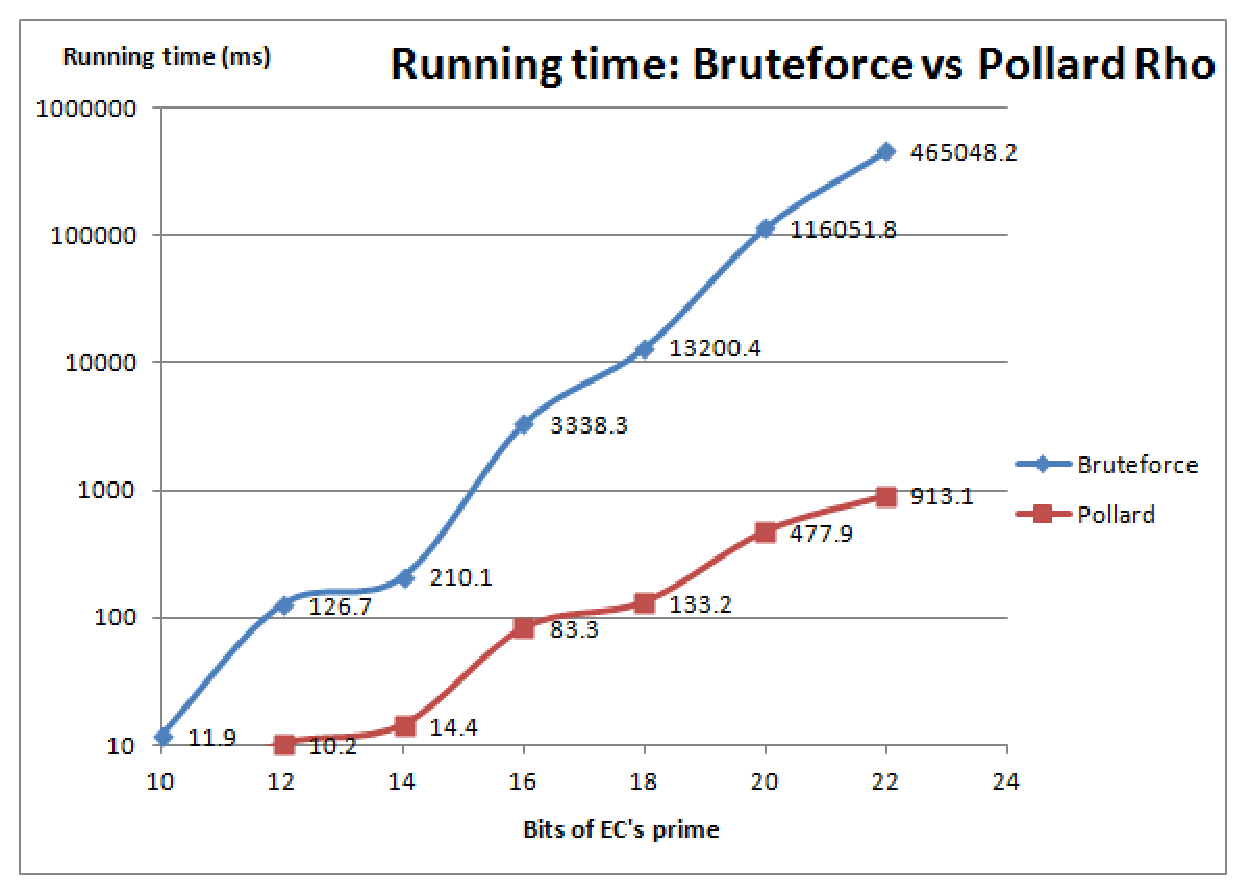
\includegraphics[scale=0.4]{runningtime_b_p.eps}
  	\caption{Running time of Bruteforce and Pollard under different bits of prime of Elliptic Curves}
  	\label{runningtime_b_p}
\end{figure}
\indent We can see that the running time is exponentially increasing when the bits of prime of the elliptic curve linearly increased. Also the speed of Pollard $\rho$ method is hundreds of times faster than Bruteforce method. \\
\indent Figure~\ref{runningtime_b2} shows the scaling up of parallelized Bruteforce method. The dataset is 20 bits primes of elliptic curves. We can see that it scales up sharply in first several times, but when thread number is near 8 the running time becomes almost the same. \\  
\indent Figure~\ref{runningtime_p2} shows the scaling up of parallelized Pollard $\rho$ method. The dataset is 22 bits primes of elliptic curves. We can see that it scales up sharply in first several times, but when thread number is near 8 the running time becomes almost the same. \\
\begin{figure}
  \centering
    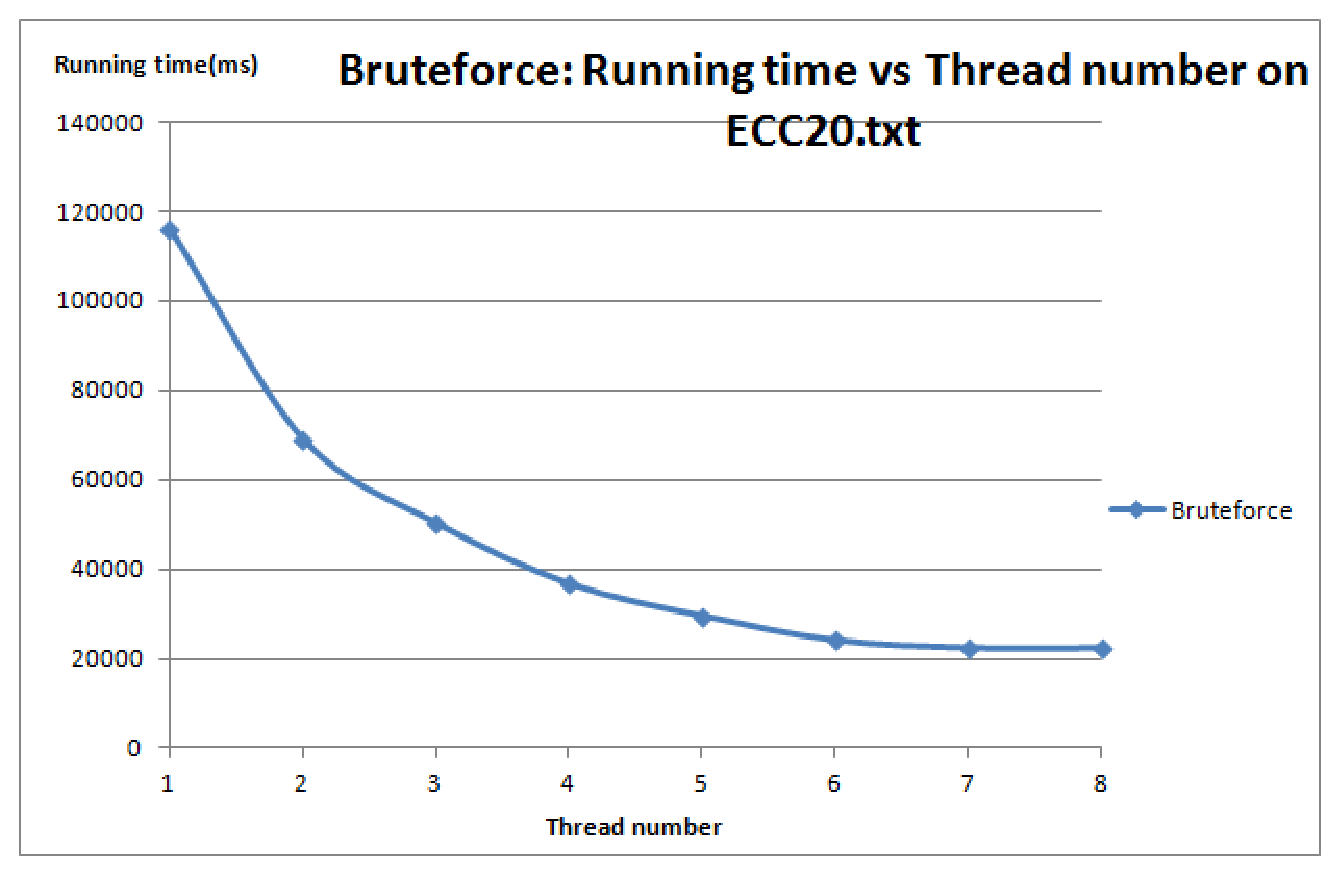
\includegraphics[scale=0.4]{runningtime_b2.eps}
  \caption{Running time of Bruteforce using different number of threads}
  \label{runningtime_b2}
\end{figure}
\begin{figure}
  \centering
    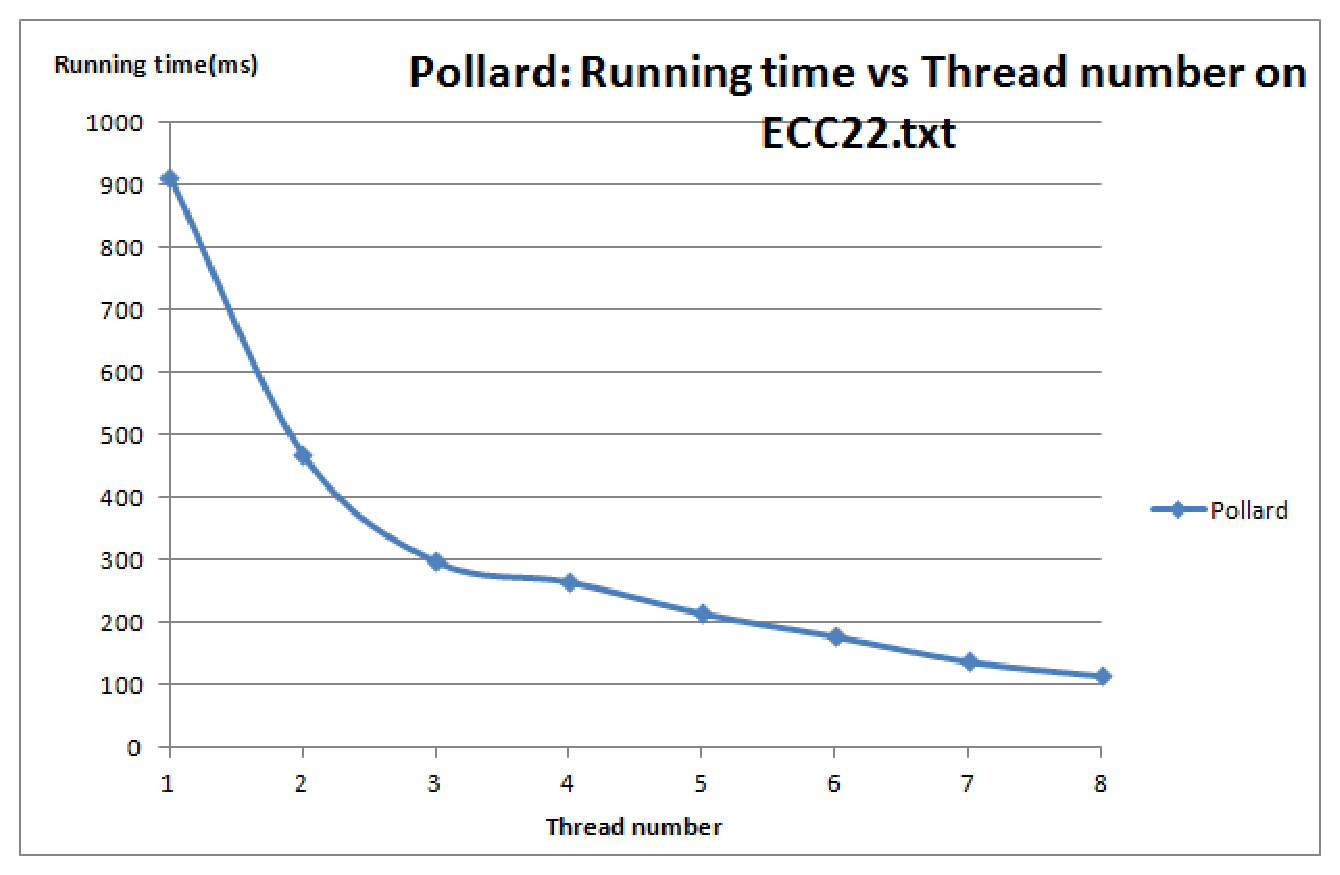
\includegraphics[scale=0.4]{runningtime_p2.eps}
  \caption{Running time of Pollard $\rho$ using different number of threads}
  \label{runningtime_p2}
\end{figure}    	
\section{Future Work}
\indent Even though we did a complete work on parallelized attacks of ECDLP, we still have many improvements can be done: \\
\indent 1. The generator now is pretty stupid. To generate a good dataset we need $O(k * n)$ time, $k$ is a constant (maybe hundreds, not trivially small) and $n$ is the same size of prime. For $t$ bits prime $n = 2^t$, which is big. \\
\indent The reason why it is so large is because it is hard to get $order(P)$. There is a much faster method called Schoof's algorithm to get $order(P)$, but it is a complicate algorithm. \\
\indent 2. The random function can be improved. Actually in \cite{CERTICOM} we can use SHA-1 to form a better random function which achieves better randomness. Better randomness may improve the speed of Pollard $\rho$ method.\\
\indent 3. We can parallelize it with more cores by using MPI and other more complicated mechanisms. 
\begin{thebibliography}{}
	\bibitem{CERTICOM} "Certicom ECC Challenge", \url{http://www.certicom.com/images/pdfs/cert_ecc_challenge.pdf}
    \bibitem{DH1976} Diffie, W. and M. Hellman, "New Directions in Cryptography", IEEE Transactions in Information Theory IT-22, pp. 644-654, 1976.	
	\bibitem{ecdsa-cert} D. Johnson, A.	Menezes and S. Vanstone, "The Elliptic Curve Digital Signature Algorithm (ECDSA)", \url{http://cs.ucsb.edu/~koc/ccs130h/notes/ecdsa-cert.pdf}
    \bibitem{E1985} ElGamal, T., "A public key cryptosystem and a signature scheme based on discrete logarithms", IEEE Transactions on Information Theory, Vol. 30, No. 4, pp. 469-472, 1985.
	\bibitem{RFC6090} D. McGrew, K. Igoe and M. Salter, "Fundamental Elliptic Curve Cryptography Algorithms", RFC6090
	\bibitem{ECC Book} L. C. Washington, "Elliptic Curves Number Theory and Cryptography", Second Edition, 2008
	\bibitem{escott.ps} A. Escott, "Implementing a
Parallel Pollard Rho Attack on ECC", \url{cacr.uwaterloo.ca/conferences/1998/ecc98/escott.ps}
    \end{thebibliography}
\end{document}
